\section {Introduction to the analysis}

In this note, we present initial results of the tracker DAQ commissioning.
\section{Description of teststand setup}
  The test stand included one DRAC card and one DTC connected to the DAQ computer,
  96 channels in total.
  The ROC was operated in the data readout mode, and the digi FPGAs were pulsed by the internal pulser.
  The pulser has two different frequencies,  31.29 MHz/(2$^7$+1), or approximately 250 kHz,
  and 31.29 MHz/(2$^9$+1), or approximately 60 kHz.
  The event window, that simulates the distance between proton pulses, could be varied by us.
  The ROC firmware has an internal hit buffer which can store up to 255 hits.
  That should be sufficient for the data taking.
  Testing therefore could proceed in two different modes:
  \begin{itemize}
  \item
    The event window is large enough , so the total number of generated hits is greater than 255. In this case
    the ROC hit buffer always gets filled up, and only the first 255 hits are read out;
  \item
    The total number of hits within the event window is less than 255.
    In this case the ROC hit buffer doesn't get filled up and the total number of hits
    can vary from one event to another.
  \end{itemize}
Pulses are created between zero and the HB and they are separated by the inverse of the generator frequency.
The event window position is uncorrelated with the generator and because of this either four or three pulses can fit in the event window.
There are channel to channel or FPGA to FPGA offsets.

\begin{figure}[!h]
\centering
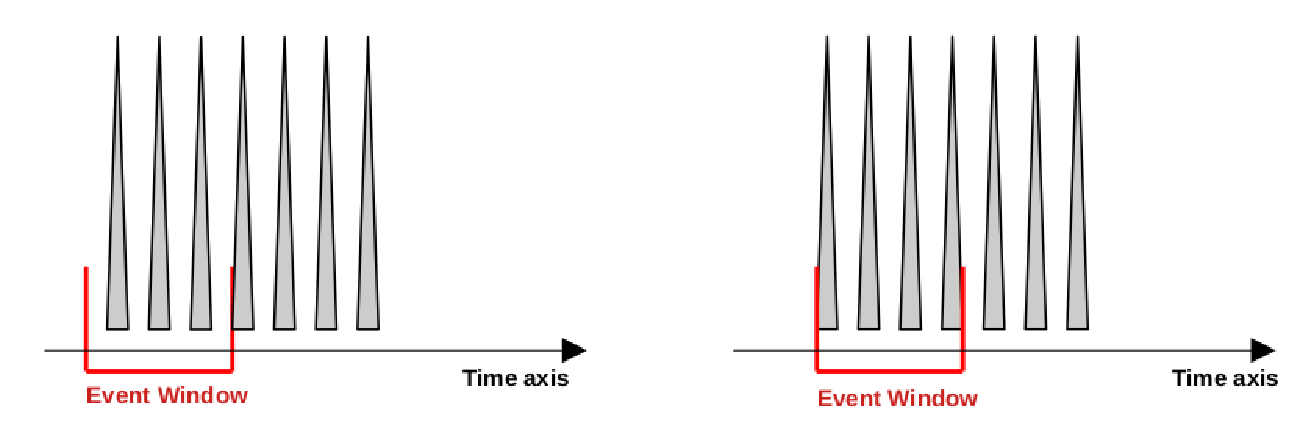
\includegraphics[width =0.8\textwidth]{figures/pdf/eventwindow}
\caption{Graphic illustration of pulses in an event window.}
\label{fig:3}
\end{figure}
\section{Monte Carlo simulation}\label{MonteCarlo}

To ensure a comprehensive understanding of our system, we initiated a Monte Carlo Simulation of our Data Acquisition (DAQ) system. 
We simulated performances of the readout logic that is purely digital, relying on different assumptions.
Given that the maximum allowable number of hits per event is 255, the simulation follows these steps:
\begin{itemize}
  \item Within a time interval ranging from zero to the HB, we generated the first event by following a uniform distribution;
    \item After verified that hits from the same channel, are separated by an interval equivalent to the reciprocal of the generator frequency, we proceeded to generate the second event by summing this specific time increment to the time of the first event;
      \item We verified whether the second pulse remained within the predefined event window. If it did, we included this hit in the ongoing event under construction;
      \item The process of event creation continued until the count of hits reached the maximum threshold of 255, at which point the event construction was terminated.
\end{itemize}
Furthermore, the simulation accounts for the channel to channel and FPGA to FPGA delays. 
This comprehensive approach ensures a faithful representation of the real-world operational aspects of the DAQ system.


%%% Local Variables:
%%% mode: latex
%%% TeX-master: t
%%% End:

